
\chapter{Cross-validation for unsupervised learning}

The problem unsupervised learning (UL) tries to to address is this: given some
data, describe its distribution. Many estimation problems can be cast as
unsupervised learning, including mean estimation, density estimation, and
linear regression. However, more commonly unsupervised learning refers to
either clustering or manifold learning. A canonical example is principal
components analysis (PCA). In PCA, we are given some high-dimensional data,
and we look for a lower-dimensional subspace that explains most of the
variation in the data. The lower-dimensional subspace describes the
distribution of the data. In clustering, the estimated cluster centers give us
information about the distribution of the data. The output of every UL method
is a summary statistic designed to convey information about the process which
generated the data.

Many UL problems involve model selection. For example, in principal components
analysis we need to choose how many components to keep. For clustering, we
need to choose the number of clusters in the data. Many manifold learning
techniques require choosing bandwidth or a kernel. Often in these contexts,
model-selection is done in an ad-hoc manner. Rules of thumb and manual
inspection guide most choices for how many components to keep, how many
clusters are present, and what is an appropriate kernel. Such informal
selection rules can be problematic when different researches come to different
conclusions about what the right model is. Moreover, even when there is an
obvious ``natural'' model to human eyes, it may be hard to pick out in
computer-automated analysis. For objectivity and efficiency, it is desirable to have a well-specified automatic model selection procedure.

For concreteness, in this chapter we focus on principal components, though
many of the ideas generalize to other methods. We suppose that the data,
$\mX$, is an $n \times p$ matrix generated according to the signal-plus-noise
model $\mX = \sqrt{n} \mU \mD \mV^\trans + \mE$. We consider the first term to
be the ``signal'' matrix, and the second term to be ``noise''. Often the
signal term is a low-rank product. Our goal is to estimate the this term as
best as possible by truncating the singular value decomposition (SVD) of
$\mX$. Here ``best'' means with respect to the metrics introduced in
Chapter~\ref{C:intrinsic-rank}. We are interested in the model selection
problem where each model is defined by the number of terms we keep from the
SVD of $\mX$.

We would like our model selection procedure to be non-parametric, if possible.
To work in a variety of contexts, the selection procedure cannot assume
Gaussianity or independence across samples. We would like the procedure to be
driven by the empirical distribution of the data. Cross-validation (CV) is a
popular approach to model selection that generally meets these criteria.
Therefore, we seek to adapt CV to our purposes.

CV prescribes dividing a data set into a ``test'' set and a
``train'' set, fitting a model to the training set, and then evaluating the
model's performance on the test set. We repeat the fit/evaluate procedure
multiple times over different test/train partitions, and then average over all
replicates. Traditionally, the partitions are chosen so that each datum occurs
in exactly one test set. As for terminology, for a particular replicate the
test set is commonly referred to as the held-out or left-out set, and likewise
the train set is often called the held-in or left-in set.

Most often, cross-validation is applied in supervised contexts. In supervised
learning (SL) the data consists of a sequence of $(\vx, \vy)$
predictor-response pairs. Broadly construed, the goal of supervised learning
is to describe the conditional distribution of $\vy$ given $\vx$. This is
usually for prediction or classification.  In the supervised context, for a
particular CV replicate there are four parts of data:
\[
    \left(
    \begin{matrix}
        \mX_\train & \mY_\train \\
        \mX_\test  & \mY_\test
    \end{matrix}
    \right).
\]
Implicit in the description of cross-validation is that the replicates use
$\mX_\test$ to predict $\mY_\test$. So, the held-in data looks like
\[
    \left(
    \begin{matrix}
        \mX_\train & \mY_\train \\
        \mX_\test  & \cdot
    \end{matrix}
    \right).
\]
We extrapolate from $\mX_\test$ to predict $\mY_\test$.

It is not immediately obvious how to apply cross-validation to unsupervised
learning.  In unsupervised learning there is no $\mY$; we instead have the
two-way partition
\[
    \left(
    \begin{matrix}
        \mX_\train \\
        \mX_\test
    \end{matrix}
    \right).
\]
There is nothing to predict!  Renaming $\mX$ to $\mY$ does not make the
problem any better, for then the division becomes:
\[
    \left(
    \begin{matrix}
        \mY_\train \\
        \mY_\test
    \end{matrix}
    \right),
\]
with hold-in
\[
    \left(
    \begin{matrix}
        \mY_\train \\
        \cdot
    \end{matrix}
    \right).
\]
There is nothing to extrapolate from to predict $\mY_\test$.  For
cross-validation to work in unsupervised learning, we need to consider
more general hold-outs.

We look at two different types of hold-outs in this chapter. The first, due to
Wold, is ``speckled'': we leave out random elements of the matrix $\mX$ and
use a missing data algorithm like expectation-maximization (EM) for
prediction. The second type of hold-out is ``blocked''. This type, due to
Gabriel, randomly partitions the columns of $\mX$ into ``predictor'' and
``response'' sets and then performs the SL version of cross-validation.


\clearpage

\begin{figure}[tbh]
    \centering
    \begin{minipage}{0.38\textwidth}
        \begin{center}
            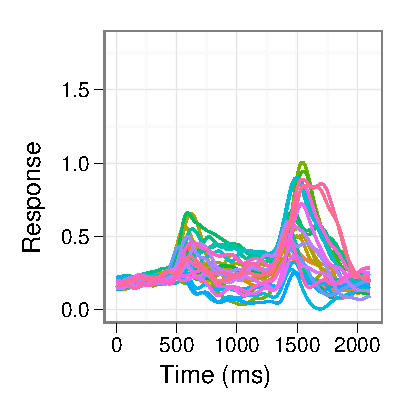
\includegraphics{neuron1}
        \end{center}
    \end{minipage}
    \begin{minipage}{0.61\textwidth}
        \begin{center}
            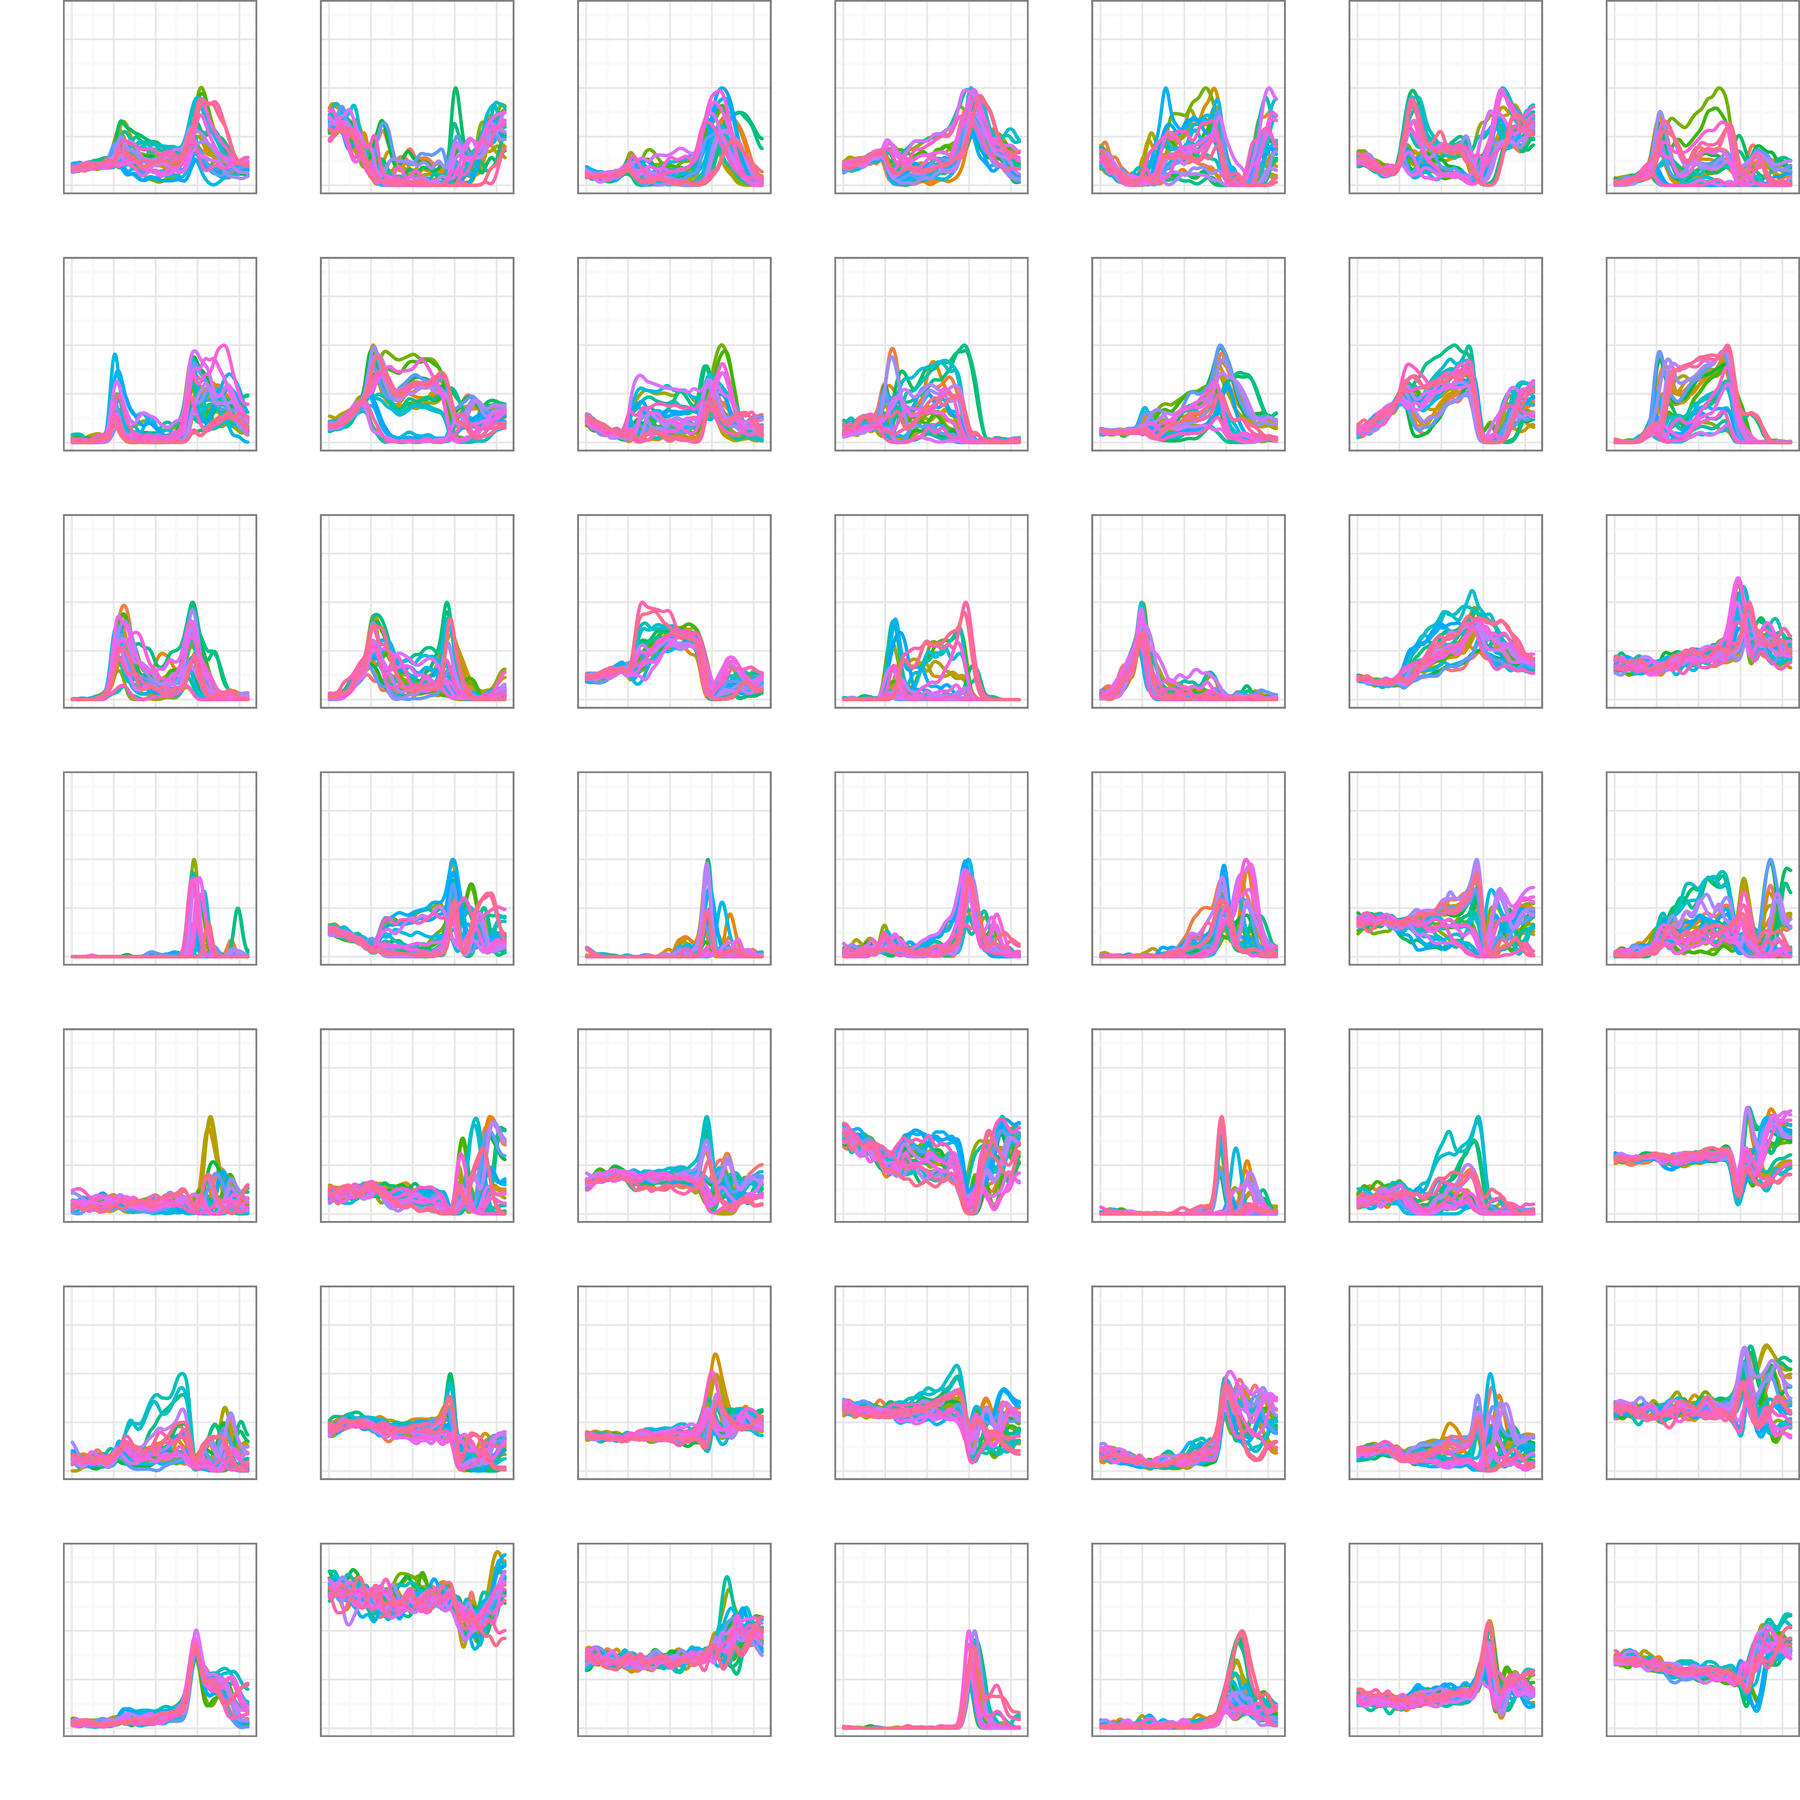
\includegraphics{neurons}
        \end{center}
    \end{minipage}
    \caption{
        \captiontitle{Motor Cortex Data}
        Response rates in 47 neurons for 27 movement tasks.  The subplots show
        the normalized response rates in a single neuron as functions of time.  
        Each color corresponds to a different movement task.  The plot on
        the left is a zoomed-in view of the data for the first neuron.
    }
\end{figure}
